\chapter{Stability, approximation and exact memory}\label{ch:stability}

The finite-mode model admits a comparatively complete stability theory under autonomous loading and integrable marks. The theory combines a branching domination, a Lyapunov function, a synchronous coupling and a small-set estimate. Kernel approximation is then controlled on a fixed horizon. Finally, exact memory reveals a sharp obstruction without feedback and a resolvent response for an associated linear system; neither statement supplies a general nonlinear stationary theory.

\begin{figure}[htb]
\centering
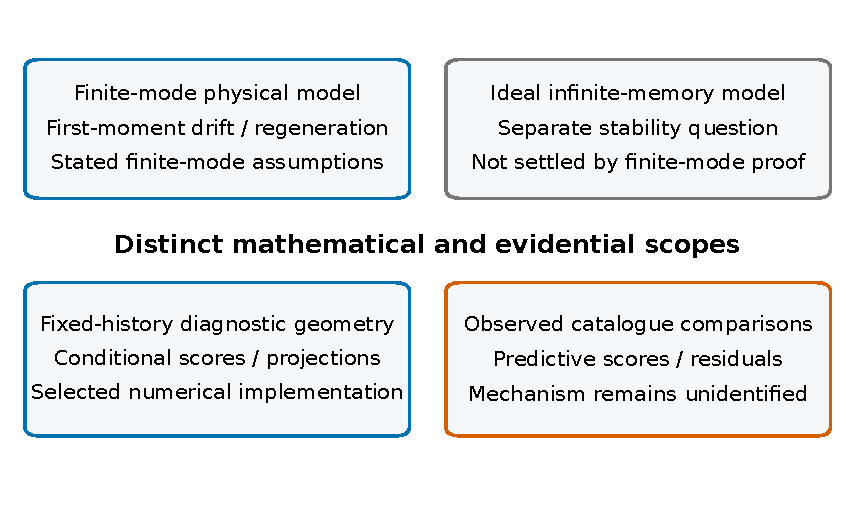
\includegraphics[width=0.95\linewidth]{theory_scope.pdf}
\caption{The positive results have different assumption sets and limiting regimes. Finite-mode invariant laws, fixed-horizon approximation and the auxiliary response do not combine into a nonlinear exact-memory ergodicity theorem.}
\label{fig:theory_scope}
\end{figure}

\section{Autonomous finite-mode stability}\label{sec:finite-stability}

Return to the physical convention \(n=\E _F\kappa(M)\). Suppose \(m_1<\infty\), \(n<1\), and \(\Psi:(-\infty,\bar x]\to(0,\infty)\) is nondecreasing and Lipschitz on the whole half-line. Write \(\bar\Psi=\Psi(\bar x)\). Put
\[
y_j=x_j^*-Z_j,\qquad Y=\sum_jw_jy_j,\qquad
W=\sum_j\frac{w_jU_j}{\vartheta_j},\qquad V=1+Y+cW,
\]
where
\begin{equation}\label{eq:c-choice}
c>\frac{m_1}{1-n}.
\end{equation}
The following theorem concerns constant \(\rho\) and fixed \(\Psi\); it is not a theorem about a time-varying diagnostic baseline.

\begin{theorem}[Finite-mode stability]\label{thm:finite_mode}
From every finite state in \(\mathcal X\), the autonomous finite-mode model has a pathwise unique, non-explosive, cadlag strong Markov construction and a Feller semigroup \(P_t\). There is a unique invariant probability \(\pi\) satisfying \(\pi(V)<\infty\). For suitable positive \(\epsilon,\beta,C,r\), with
\[
\|z-z'\|=\sum_jw_j\bigl(|Z_j-Z'_j|+|U_j-U'_j|\bigr),\qquad
d_\epsilon(z,z')=1\wedge\frac{\|z-z'\|}{\epsilon},
\]
and
\[
\widetilde d(z,z')=
\sqrt{d_\epsilon(z,z')\{1+\beta V(z)+\beta V(z')\}},
\]
one has
\begin{equation}\label{eq:weighted-contraction}
W_{\widetilde d}(P_t(z,\cdot),\pi)
\leq Ce^{-rt}\sqrt{1+V(z)},\qquad t\geq0.
\end{equation}
In particular, \(P_t(z,\cdot)\) converges weakly to \(\pi\).
\end{theorem}

Here \(W_c\) is the infimum of the expected cost \(c\) over couplings. The weighted cost \(\widetilde d\) need not satisfy a triangle inequality; the conclusion is not a total-variation mixing statement.

The constants generally depend on the rates, weights, \(m_1\), \(n\), the Lipschitz constant of \(\Psi\) and \(\bar\Psi\). No uniformity is claimed as \(\vartheta_{\min}=\min_j\vartheta_j\) tends to zero; the contractive time and the selected radius may deteriorate in that limit.

\begin{proof}
\emph{Construction and nonexplosion.} Use a marked Poisson embedding with thinning by the predictable intensity \(\Psi(X)+H\). The process is dominated by a marked Hawkes process with immigration \(\bar\Psi\), kernel
\[
h_d(t)=\sum_jw_j\vartheta_je^{-\vartheta_jt},
\]
and initial excitation \(\sum_jw_jU_j(0)e^{-\vartheta_jt}\). The latter integrates to \(W(z)\), and each cluster has expected total size \(1/(1-n)\). For every nonnegative mark weight \(\omega\) with finite mean,
\begin{equation}\label{eq:cluster-moment}
\E _z\sum_{T_i\leq T}\omega(M_i)
\leq\frac{\E _F\omega(M)}{1-n}
\{\bar\Psi T+W(z)\}.
\end{equation}
A generation is created before its marks are drawn, so \eqref{eq:cluster-moment} remains valid when \(\omega\) and \(\kappa\) are correlated. Finite expected counts imply nonexplosion; the deterministic flow and fresh Poisson increments yield the strong Markov property.

\emph{Lyapunov estimate.} Since the flow gives \(\dot Y=-\sum_jw_j\vartheta_jy_j\) and \(\dot W=-H\), while a jump adds \((g,\kappa)\), the extended generator satisfies
\[
\mathcal AV
=-\sum_jw_j\vartheta_jy_j-\delta H+(m_1+cn)\Psi(X),
\qquad
\delta=c(1-n)-m_1>0.
\]
Because \(\Psi(X)\leq\bar\Psi\) on \(\mathcal X\), direct comparison with the positive relaxation terms gives
\begin{equation}\label{eq:generator-bound}
\mathcal AV\leq-\omega V+D,
\end{equation}
where
\[
K_0=(m_1+cn)\bar\Psi,\qquad
\omega=\vartheta_{\min}\min\{1,\delta/c\},\qquad
D=\omega+K_0.
\]
The weighted jump bound \eqref{eq:cluster-moment} makes the stopped compensated jump integral integrable. Applying the product formula to \(e^{\omega t}V(z_t)\) and then Fatou's lemma gives
\begin{equation}\label{eq:lyap-moment}
P_tV(z)\leq e^{-\omega t}V(z)+\frac{D}{\omega}(1-e^{-\omega t}).
\end{equation}

\emph{Coupling and smallness.} Couple two copies synchronously until their first unmatched event \(\sigma\). Identical jumps cancel before \(\sigma\), so
\[
\|z_t-z'_t\|\leq e^{-\vartheta_{\min}t}\|z-z'\|
\]
on \(\{\sigma>t\}\). Bounding the compensator of the difference of their rates by \(L\|z_t-z'_t\|\), with \(L=\max\{L_\Psi,1\}\), gives
\[
\mathbb P(\sigma\leq t)\leq
\frac{L}{\vartheta_{\min}}\|z-z'\|.
\]
Thus, whenever \(d_\epsilon(z,z')<1\),
\begin{equation}\label{eq:coupling-contraction}
W_{d_\epsilon}(P_tz,P_tz')
\leq\left(e^{-\vartheta_{\min}t}
+\frac{L\epsilon}{\vartheta_{\min}}\right)d_\epsilon(z,z').
\end{equation}
Choose \(\epsilon\) small and then \(t\) large enough to make the coefficient less than one up to the prescribed margin. Sublevel sets \(\{V\leq R\}\) are compact and have finite diameter \(D_R\). On such a set, event-free flow decreases both \(Y\) and \(W\), and the event rate is at most \(\Lambda_R=\bar\Psi+\vartheta_{\max}R/c\). 
Use the same marked Poisson random measure $\Pi$ for both
copies, with intensity $\dif s\,\dif u\,F(\dif m)$ and the
usual acceptance threshold. The event
\[
 \Pi\bigl([0,t]\times[0,\Lambda_R]\times\mathsf M\bigr)=0
\]
has probability $e^{-\Lambda_Rt}$, since $F$ has total mass one. On this
event both copies follow their event-free flows and their rates remain at
most $\Lambda_R$, so neither jumps. Thus the synchronous coupling gives probability at least $e^{-\Lambda_Rt}$ that neither copy jumps. Once \(e^{-\vartheta_{\min}t}D_R\leq\epsilon/2\),
\[
\sup_{V(z),V(z')\leq R}W_{d_\epsilon}(P_tz,P_tz')
\leq1-\tfrac12e^{-\Lambda_Rt}<1.
\]
The same coupling shows that the state at a fixed time converges in probability as the initial state varies continuously. Expectations of bounded continuous functions therefore converge, establishing the Feller property. To choose a common time for contraction and smallness, first fix \(R=4D/\omega\) from the Lyapunov bound, then choose time sufficiently large for both inequalities.

Together with \eqref{eq:lyap-moment} this verifies the Lyapunov, contraction and smallness hypotheses of \citet{HairerMattinglyScheutzow2011}, Theorem~4.8 in the author-final version. Their Corollary~4.11 adds existence under the Feller and completeness conditions used here. Existence also follows from tight time-averaged laws, compact sublevels and \eqref{eq:lyap-moment}. The contraction time provided by the theorem may be later than the time used to check the hypotheses. Replacing \(d_\epsilon\) by \(\widetilde d\) and iterating the resulting contraction, while using \eqref{eq:lyap-moment} for the residual time, gives \eqref{eq:weighted-contraction}. No second mark moment is required.

To see that every invariant probability has the same finite moment without subtracting potentially infinite integrals, suppose \(PV\leq aV+b\) with \(a<1\), and put \(f_K(v)=\min(v,K)\). If \(\nu\) is invariant, concavity gives
\[
\nu\{f_K(V)-f_K(aV+b)\}\leq0.
\]
For \(K\geq b/(1-a)\), the integrand is at least
\([(1-a)V-b]\mathbf 1_{\{V\leq K\}}\). Hence
\(\nu(V\mathbf 1_{\{V\leq K\}})\leq b/(1-a)\). Monotone convergence and \eqref{eq:lyap-moment} yield \(\nu(V)\leq D/\omega\). The weak Harris theorem supplies uniqueness.
\end{proof}

Under the invariant law, let \(\Lambda=\pi(\Psi(X)+H)>0\). Stationarity in the coordinate equations, justified by the weighted jump bound, gives
\[
\pi(U_j)=n\Lambda,\qquad
\pi(Z_j)=\frac{\rho-m_1\Lambda}{\vartheta_j},\qquad
\Lambda=\frac{\pi(\Psi(X))}{1-n},
\]
and hence
\[
\pi(X)=(\rho-m_1\Lambda)\sum_j\frac{w_j}{\vartheta_j}.
\]
Under \(\mathbb P_\pi\), intensity ergodicity and the compensated counting martingale give \(N(t)/t\to\Lambda\), while the fresh-mark strong law gives \(t^{-1}\sum_{T_i\leq t}g(M_i)\to m_1\Lambda\).

\begin{proposition}[Infinite stationary second moments]\label{prop:heavy-moments}
If \(\E _Fg(M)^2=\infty\), then \(\pi(Y^2)=\infty\) and consequently \(\pi(X^2)=\infty\). If \(\E _F\kappa(M)^2=\infty\), then \(\pi(W^2)=\infty\) and consequently \(\pi(H^2)=\infty\).
\end{proposition}

\begin{proof}
Let \(\Phi_d(t)=\sum_jw_je^{-\vartheta_jt}>0\). The mild equations for the nonnegative depletion modes \(y_j\) and the integrated excitation modes give, on any stationary interval of length \(t\),
\[
Y(0)^2\geq\Phi_d(t)^2\sum_{-t<T_i\leq0}g(M_i)^2,
\qquad
W(0)^2\geq\Phi_d(t)^2\sum_{-t<T_i\leq0}\kappa(M_i)^2.
\]
Replace a squared mark by \(g_K^2=(g\wedge K)^2\). Fresh-mark compensation, applied before each mark is revealed, gives
\[
\E _\pi\sum_{-t<T_i\leq0}g_K(M_i)^2
=\E _Fg_K(M)^2\int_{-t}^0\E _\pi\lambda_s\,\dif s
=t\Lambda\E _Fg_K(M)^2.
\]
Thus
\(\pi(Y^2)\geq\Phi_d(t)^2t\Lambda\E _Fg_K(M)^2\).
Letting \(K\uparrow\infty\) proves the first implication. The productivity argument is identical. Since \(X=\bar x-Y\), infinite \(\pi(Y^2)\) implies infinite \(\pi(X^2)\). Since \(W\) and \(H\) are comparable through the finitely many positive rates, infinite \(\pi(W^2)\) implies infinite \(\pi(H^2)\).
\end{proof}

The argument concerns the corresponding jump transform: it asserts stress divergence when the stress-mark second moment diverges, and excitation divergence when the productivity second moment diverges. Finite first-moment stability and infinite stationary variance coexist. A quadratic theorem under stronger finite-moment assumptions is not contradicted; those stronger assumptions cannot be inferred for an untruncated heavy-tailed fitted law.

\section{Fixed-horizon kernel approximation}

Let \(\Phi\) and \(\Phi_d\) be nonnegative decreasing absolutely continuous kernels, normalised to one at zero and tending to zero at infinity, so that \(h=-\Phi'\) and \(h_d=-\Phi_d'\) are probability densities. Use the same finite initial stress and constant loading, no prehistory, fresh marks, and the first-moment assumptions above. Let \(\Psi\) be positive, nondecreasing and locally Lipschitz on \(\mathbb R\). For fixed \(T<\infty\), put
\[
B=A_T=|X_0|+\rho T,\qquad
K_T=\frac{\Psi(B)T}{1-n},
\]
\[
\Delta_\Phi=\sup_{[0,T]}|\Phi_d-\Phi|,
\qquad
\Delta_h=\int_0^T|h_d-h|.
\]

\begin{proposition}[Quantitative half-line approximation]\label{prop:quantitative-kernel}
If \(\Psi\) is Lipschitz on \((-\infty,B]\) with constant \(L_B\), then, under the same Poisson-measure coupling,
\begin{equation}\label{eq:quantitative-kernel}
\mathbb P(\text{marked catalogues differ on }[0,T])
\leq\min\{1,\;L_BT(A_T+m_1K_T)\Delta_\Phi+nK_T\Delta_h\}.
\end{equation}
For \(\Psi(x)=e^{a+bx}\), \(b\geq0\), one may take \(L_B=be^{a+bB}\).
\end{proposition}

\begin{proof}
All stresses remain at most \(B\). Until the two coupled processes first separate,
\[
|X_d(s)-X(s)|
\leq\Delta_\Phi\left(A_T+\sum_{T_i<s}g(M_i)\right),
\]
and the integrated excitation discrepancy is bounded by
\(\Delta_h\sum_{T_i\leq T}\kappa(M_i)\). Common pre-separation events form a subset of the reference events, which are dominated by the Hawkes process with immigration \(\Psi(B)\). Its expected event count is at most \(K_T\), while the corresponding weighted expectations are at most \(m_1K_T\) and \(nK_T\). Bounding the compensated difference of the two event intensities by the stress discrepancy and the excitation discrepancy and integrating its expectation gives \eqref{eq:quantitative-kernel}.
\end{proof}

Local Lipschitz continuity does not support the same linear error bound. It nevertheless gives qualitative convergence through a separate truncation.

\begin{proposition}[Qualitative local approximation]\label{prop:qualitative-kernel}
For \(R>0\), let \(L_R\) be a Lipschitz constant of \(\Psi\) on \([-|X_0|-R,B]\). Then
\begin{equation}\label{eq:qualitative-kernel}
\mathbb P(\text{catalogues differ on }[0,T])
\leq\min\left\{1,\frac{m_1K_T}{R}
+L_RT(A_T+R)\Delta_\Phi+nK_T\Delta_h\right\}.
\end{equation}
\end{proposition}

\begin{proof}
On common prehistories whose cumulative release is at most \(R\), both stresses lie in the compact interval on which \(L_R\) is valid, and the half-line calculation applies with \(R\) in place of the full released mass. The complement has probability at most \(m_1K_T/R\) by Markov's inequality. Fix \(R\), let the two kernel errors tend to zero, and then let \(R\to\infty\).
\end{proof}

Thus half-line Lipschitz continuity gives a quantitative error rate, whereas local Lipschitz continuity gives only qualitative fixed-horizon convergence. A finite half-line constant cannot be inferred from local Lipschitz continuity. Nor do these results exchange the kernel-approximation and long-time limits.

\section{Exact-memory obstruction and response}

Exact memory neither prevents all stationary constructions nor yields a general nonlinear stationary theorem. The first point is visible already in a zero-history model without feedback.

\begin{proposition}[No-feedback obstruction]\label{prop:exact-obstruction}
Let \(0<\alpha<1\), \(\tau>0\), and
\(\Phi(t)=E_\alpha(-(t/\tau)^\alpha)\). Consider the zero-history model with \(X_0=0\), constant immigration rate \(\mu>0\), no triggering, and loading \(\rho=\mu\E  S\). Let \(N(\dif v,\dif S)\) be Poisson with intensity \(\mu\,\dif v\,F_S(\dif S)\), let \(\widetilde N\) be its compensated measure, and define
\[
X(t)=-\int_0^t\Phi(t-v)S\,\widetilde N(\dif v,\dif S).
\]
If \(S=1\), no sequence \(t_k\to\infty\) has a tight subsequence of stress laws for \(\alpha\leq1/2\). If \(P(S>s)=s^{-q}\) for \(s\geq1\) and \(1<q<2\), the corresponding obstruction occurs when \(\alpha q\leq1\). For \(S=1\), \(\alpha>1/2\) admits a stationary two-sided compensated moving average in \(L^2\), and the zero-history one-time laws converge. For Pareto marks, \(\alpha q>1\) admits such a construction in \(L^p\) for every \(1/\alpha<p<q\).
\end{proposition}

\begin{proof}
The finite-interval Poisson exponential formula gives
\begin{equation}\label{eq:obstruction-cf}
\left|\E  e^{iuX(t)}\right|
=\exp\left\{-\mu\int_0^t
\E _F\{1-\cos(uS\Phi(v))\}\,\dif v\right\}.
\end{equation}
For unit marks, the integrand is asymptotic to \(u^2\Phi(v)^2/2\) for fixed \(u\neq0\). For Pareto marks and \(0<x\leq1\), restricting \(S\) to \([1/x,2/x]\) yields
\[
\E _F\{1-\cos(xS)\}
\geq(1-\cos1)(1-2^{-q})x^q.
\]
Since
\(\Phi(v)\sim\tau^\alpha v^{-\alpha}/\Gamma(1-\alpha)\),
the modulus \eqref{eq:obstruction-cf} tends to zero at every nonzero frequency in the stated regimes. Tightness would give a weak subsequential limit; by the continuity theorem its characteristic function would be continuous at zero, but the limit would equal zero at every \(u\neq0\) and one at \(u=0\), a contradiction.

Above the threshold, the two-sided compensated integrals converge in \(L^2\) by the isometry for unit marks. For Pareto marks, choose \(1/\alpha<p<q\). Then \(\E  S^p<\infty\) and \(\int_0^\infty\Phi(v)^p\,\dif v<\infty\), so the compensated Poisson \(L^p\) estimate gives the two-sided construction.
\end{proof}

This is a no-feedback statement. It does not assert nonstationarity of the stress-sensitive nonlinear model, and a stationary compensated construction is not the subtraction of two separately divergent, uncompensated past integrals.

For an auxiliary excitation-inclusive system, a positive stress-to-rate slope changes the response through an integrable resolvent with a heavy tail. Let \(m_1>0\), \(0\leq n<1\) and \(\ell>0\), and consider
\begin{equation}\label{eq:aux-response-equations}
x=-m_1\Phi*y,\qquad
y=\ell x+nh*y+\xi,\qquad
h=-\Phi',
\end{equation}
with zero initial perturbation and additive event-flux forcing \(\xi\). Set
\[
\gamma=m_1\ell,\qquad \beta_{\mathrm{rel}}=1-\alpha,\qquad
a_{\mathrm{rel}}=(1-n)\tau^{-\alpha}.
\]

\begin{proposition}[Excitation-inclusive response]\label{prop:auxiliary-response}
The causal solution of \eqref{eq:aux-response-equations} is
\(x=-m_1R_\gamma*\xi\), where
\begin{equation}\label{eq:response-transform}
\widehat R_\gamma(s)=\frac{1}{s+a_{\mathrm{rel}} s^{\beta_{\mathrm{rel}}}+\gamma}.
\end{equation}
For \(\gamma>0\), \(R_\gamma\) is completely monotone, \(R_\gamma(0+)=1\), \(\int_0^\infty R_\gamma(t)\,\dif t=1/\gamma\), and
\begin{equation}\label{eq:response-tail}
R_\gamma(t)\sim
\frac{a_{\mathrm{rel}}\beta_{\mathrm{rel}}}{\gamma^2\Gamma(1-\beta_{\mathrm{rel}})}t^{-1-\beta_{\mathrm{rel}}}.
\end{equation}
In particular, \(\int_0^\infty tR_\gamma(t)\,\dif t=\infty\).
\end{proposition}

\begin{proof}
Eliminating \(y\) in the Laplace domain gives
\[
\widehat\Phi(s)=\frac{s^{\alpha-1}}{s^\alpha+\tau^{-\alpha}},
\qquad
\widehat h(s)=\frac{\tau^{-\alpha}}{s^\alpha+\tau^{-\alpha}}.
\]
Substitution into \eqref{eq:aux-response-equations} yields
\[
\widehat x(s)=-\frac{m_1s^{\alpha-1}\widehat\xi(s)}
{s^\alpha+\gamma s^{\alpha-1}+(1-n)\tau^{-\alpha}}
=-m_1\widehat R_\gamma(s)\widehat\xi(s),
\]
which is \eqref{eq:response-transform}. The reciprocal of the nonnegative complete Bernstein function \(s+a_{\mathrm{rel}} s^{\beta_{\mathrm{rel}}}+\gamma\) is a Stieltjes function, hence \(R_\gamma\) is completely monotone
\citep[Section~2.1]{MeerschaertToaldo2019}. Its spectral density is
\[
k_\gamma(r)=
\frac{a_{\mathrm{rel}}\sin(\pi\beta_{\mathrm{rel}})r^{\beta_{\mathrm{rel}}}}
{\pi\{[\gamma-r+a_{\mathrm{rel}} r^{\beta_{\mathrm{rel}}}\cos(\pi\beta_{\mathrm{rel}})]^2+
a_{\mathrm{rel}}^2r^{2\beta_{\mathrm{rel}}}\sin^2(\pi\beta_{\mathrm{rel}})\}},
\]
so \(R_\gamma(t)=\int_0^\infty e^{-rt}k_\gamma(r)\,\dif r\). The limits of \eqref{eq:response-transform} at infinity and zero give \(R_\gamma(0+)=1\) and \(\int R_\gamma=1/\gamma\). Near \(r=0\),
\[
k_\gamma(r)\sim
\frac{a_{\mathrm{rel}}\sin(\pi\beta_{\mathrm{rel}})}{\pi\gamma^2}r^{\beta_{\mathrm{rel}}}.
\]
Rescaling the spectral integral and using the gamma reflection formula gives \eqref{eq:response-tail}. The tail exponent \(-1-\beta_{\mathrm{rel}}\) lies between \(-2\) and \(-1\), so the first temporal moment diverges.
\end{proof}

The weak-feedback crossover is equally explicit. Put \(t_\gamma=(a_{\mathrm{rel}}/\gamma)^{1/\beta_{\mathrm{rel}}}\). As \(\gamma\downarrow0\), the probability densities \(\gamma t_\gamma R_\gamma(t_\gamma u)\) on \((0,\infty)\) converge weakly to the law with Laplace transform \((1+z^{\beta_{\mathrm{rel}}})^{-1}\), because
\[
\int_0^\infty e^{-zu}\gamma t_\gamma R_\gamma(t_\gamma u)\,\dif u
=\frac{1}{1+z^{\beta_{\mathrm{rel}}}+z/(\gamma t_\gamma)}
\longrightarrow\frac{1}{1+z^{\beta_{\mathrm{rel}}}}.
\]
At \(\gamma=0\), \(R_0(t)=E_\alpha(-a_{\mathrm{rel}}t^\alpha)\) is not integrable. The crossover is separated from the early-time scale \(a_{\mathrm{rel}}^{-1/\alpha}\) only when \(\gamma\ll a_{\mathrm{rel}}^{1/\alpha}\). This is a statement about an auxiliary impulse response, not a nonlinear mixing time.

A restricted nonlinear observation follows from the same resolvent. For
\[
y=\psi(x)+nh*y+\xi,\qquad \psi(0)=0,
\]
write \(\mathcal E(x)=m_1\psi(x)-\gamma x\). If \(\mathcal E\) is globally Lipschitz with constant \(L<\gamma\), the equivalent map
\[
x=-R_\gamma*(m_1\xi+\mathcal E(x))
\]
is a contraction on bounded causal functions, and
\(\|x\|_\infty\leq m_1\|\xi\|_\infty/(\gamma-L)\). This is only an externally forced auxiliary Volterra result. The positive exponential rate does not satisfy such a global sector condition, since its derivative tends to zero as stress tends to negative infinity. For jointly measurable stationary forcing with an almost surely uniform deterministic bound, the integrable-resolvent fixed-point equation has a unique bounded causal stationary solution by contraction and shift-equivariant Picard iteration, but it does not assert absolute convergence of the two-sided convolution \(\Phi*y\), because \(\Phi\) is not integrable.

The obstruction and resolvent calculation therefore delimit the demonstrated scope. Neither supplies a generic stationary theorem for the nonlinear stress-sensitive exact-memory process.

\subsection{What the auxiliary response omits}

The actual marked process has two noise sources rather than a single prescribed event-flux input. In the physical productivity convention, define compensated marked measures by
\[
\dif M_g=\dif N_g-m_1\lambda\,\dif t,\qquad
\dif M_\kappa=\dif N_\kappa-n\lambda\,\dif t,
\]
where $N_g$ and $N_\kappa$ accumulate the corresponding marks. These martingales are generally correlated: both jump at the same events, and the two transforms of a fresh mark need not be independent. 

\begin{samepage}
Set $Q_\gamma=R_\gamma-nR_\gamma*h$, and let $X^+(t)$ denote post-event stress, including releases at time $t$. For scalar initial stress \(X_0\Phi(t)\), zero initial excitation and no additional prehistory, finite-horizon compensation and the same Laplace-resolvent algebra give the exact identity
\begin{align}
X^+(t)={}&X_0Q_\gamma(t)+\rho\int_0^tQ_\gamma(u)\,\dif u \notag\\
&+[R_\gamma*(\gamma X^+-m_1\Psi(X^+_-))](t) \notag\\
&-\int_{(0,t]}Q_\gamma(t-u)\,\dif M_g(u) \notag\\
&-m_1\int_{(0,t]}(R_\gamma*h)(t-u)\,\dif M_\kappa(u).
\label{eq:marked-resolvent}
\end{align}
\end{samepage}
Here $X^+_-(u)=X^+(u^-)$, and all assertions are on finite horizons under compensator integrability. At an event time, the intensity uses the left limit; the displayed post-event identity must be left-limited consistently if it is used to evaluate that intensity. The deterministic kernels in the two noise terms are bounded and integrable, but this does not by itself control the nonlinear residual in the second line. In particular, the stress can leave any band on which a positive lower slope is available. Establishing tightness or a uniform occupation bound outside that band remains a separate task. The identity explains the relevance of the auxiliary response while retaining the nonlinear term and both correlated mark martingales.

\paragraph{Compensation and cancellation.}
An event-free path has $\dif N_g=\dif N_\kappa=0$, but not
$\dif M_g=\dif M_\kappa=0$. Instead,
\[
  \dif M_g=-m_1\lambda\,\dif t,
  \qquad
  \dif M_\kappa=-n\lambda\,\dif t.
\]
The compensated integrals must therefore be retained even when no event
occurs. The causal kernels satisfy
\[
 Q_\gamma+nR_\gamma*h=R_\gamma,
 \qquad
 Q_\gamma+\gamma R_\gamma*\Phi=\Phi.
\]
For the stated initialization, put
$f=X_0\Phi+\rho(1*\Phi)$, where $(1*\Phi)(t)=\int_0^t\Phi(u)\,\dif u$.
In the following ordinary time convolutions write $X$ for $X^+$, retaining
$X_-$ in the predictable intensity. The original equations give
\[
 X=f-\Phi*\dif N_g,
 \qquad \lambda=\Psi(X_-)+h*\dif N_\kappa.
\]
Substitution of both compensated measures into the displayed identity,
followed by the first kernel relation, reduces its right-hand side to
\[
 X_0Q_\gamma+\rho(1*Q_\gamma)-Q_\gamma*\dif N_g
   +\gamma R_\gamma*X.
\]
The second kernel relation makes the first three terms
$X-\gamma R_\gamma*X$, proving the cancellation. These are finite-horizon
causal convolution identities under the stated integrability conditions;
no infinite-history transform of a nonlinear sample path or stationary
exact-memory limit is asserted.

The worked event-free example and expanded derivations are provided in the new explanatory supplement E04, \path{supplements/explanatory_supplement.pdf}.

The stationary balance of finite mixtures provides only a conditional further observation. If $A_d=\int_0^\infty\Phi_d(t)\dif t\to\infty$, $m_1>0$, and their invariant means satisfy $\sup_d|\E _{\pi_d}X_d|<\infty$, then
\[
\E _{\pi_d}X_d=(\rho-m_1\Lambda_d)A_d
\quad\Longrightarrow\quad
m_1\Lambda_d\longrightarrow\rho.
\]
The assumed uniform bound is precisely what the fixed-mode theorem does not supply. This consequence cannot establish convergence of invariant laws or justify interchanging the mode and stationary limits.


